\documentclass[12pt,a4paper]{scrartcl}
\usepackage[utf8]{inputenc}
\usepackage[english,russian]{babel}
\usepackage{indentfirst}
\usepackage{misccorr}
\usepackage{graphicx}
\usepackage{amsmath}
\usepackage{multirow}
\usepackage{pgfplots}
\usepackage{parskip}
\usepackage[top=1cm, bottom=1cm, left=1cm, right=1cm]{geometry}
\pgfplotsset{compat=1.9}

\begin{document}
	\graphicspath{{py/}}
	
	\newcommand{\ms}{\mathstrut}
	\newcommand{\msp}{\hspace{0.5cm}}
	\newcommand{\al}{\alpha}
	\newcommand{\dg}{^\circ}
	\newcommand{\dif}{\mathrm{d}}
	\newcommand{\qd}[2]{^{\frac{#1}{#2}}}
	\newcommand{\qdm}[2]{^{-\frac{#1}{#2}}}
	\newcommand{\lm}[2]{\underset{#1 \rightarrow #2}{\lim}}
	\newcommand{\sfrac}[2]{\dfrac{\strut #1}{\strut #2}}
	\newcommand{\equal}[1]{\overset{(#1)}{=}}
	\newcommand{\linevdots}{\ \raisebox{-.08\height}{\vdots}\ }
	\newcommand{\linecvdots}{\ \raisebox{-.08\height}{\vdots}\hspace{-0.13cm}\raisebox{.15\height}{\cancel{\phantom{a}}\hspace{0.06cm}}}
	\newcommand{\combox}[1]{\ms \msp \msp \begin{minipage}{0.95\linewidth}
			#1
	\end{minipage}}
	
	\newtheorem{pr}{Задача}
	\newtheorem{ex}{Пример}
	\newtheorem{dfn}{Def}
	\newtheorem{theorem}{Th}
	
	\newenvironment{slv}{\ms \msp \textit{Решение:}}{}
	\newenvironment{proof}{\ms \msp \textit{Доказательство: }}{\hfill $\square$}
	
	\begin{titlepage}
		
		\vspace*{\fill}
		
		\begin{center}
			
\includegraphics[scale=0.8]{MIPT.png}
			\\[0.7cm]\Huge Московский Физико-Технический Институт\\(национальный исследовательский университет)
			\\[2cm]\LARGE Отчет по эксперименту
			\\[0.5cm]\noindent\rule{\textwidth}{1pt}
			\\\Huge\textbf{Эффект Джоуля-Томсона}
			\\[-0.5cm]\noindent\rule{\textwidth}{1pt}
		\end{center}
		
		\begin{flushleft}
			\textit{Работа №2.1.6; дата: 06.05.22}\hfill\textit{Семестр: 2}
		\end{flushleft}
		
		\vspace*{\fill}
		
		\begin{flushleft}
			Выполнил: \hspace{\fill} Группа:
			\\Кошелев Александр \hspace{\fill} Б05-105
		\end{flushleft}
	\end{titlepage}
	
	%Страница 2
	
	\begin{flushleft}
		\footnotesize{Эффект Джоуля-Томсона} \hspace{\fill} \footnotesize{2}
		\\[-0.3cm]\noindent\rule{\textwidth}{0.3pt}
	\end{flushleft}
	
	\section{Аннотация}
	
	\textbf{Цель работы: }
	
	\begin{enumerate}
		\item Определение изменения температуры углекисло-
		го газа при протекании через малопроницаемую перегородку при
		разных начальных значениях давления и температуры;
		\item Вычисление по результатам опытов коэффициентов Ван-дер-Ваальса $a$ и
		$b$.
	\end{enumerate}
	
	\textbf{Схема установки:}
	\begin{center}
		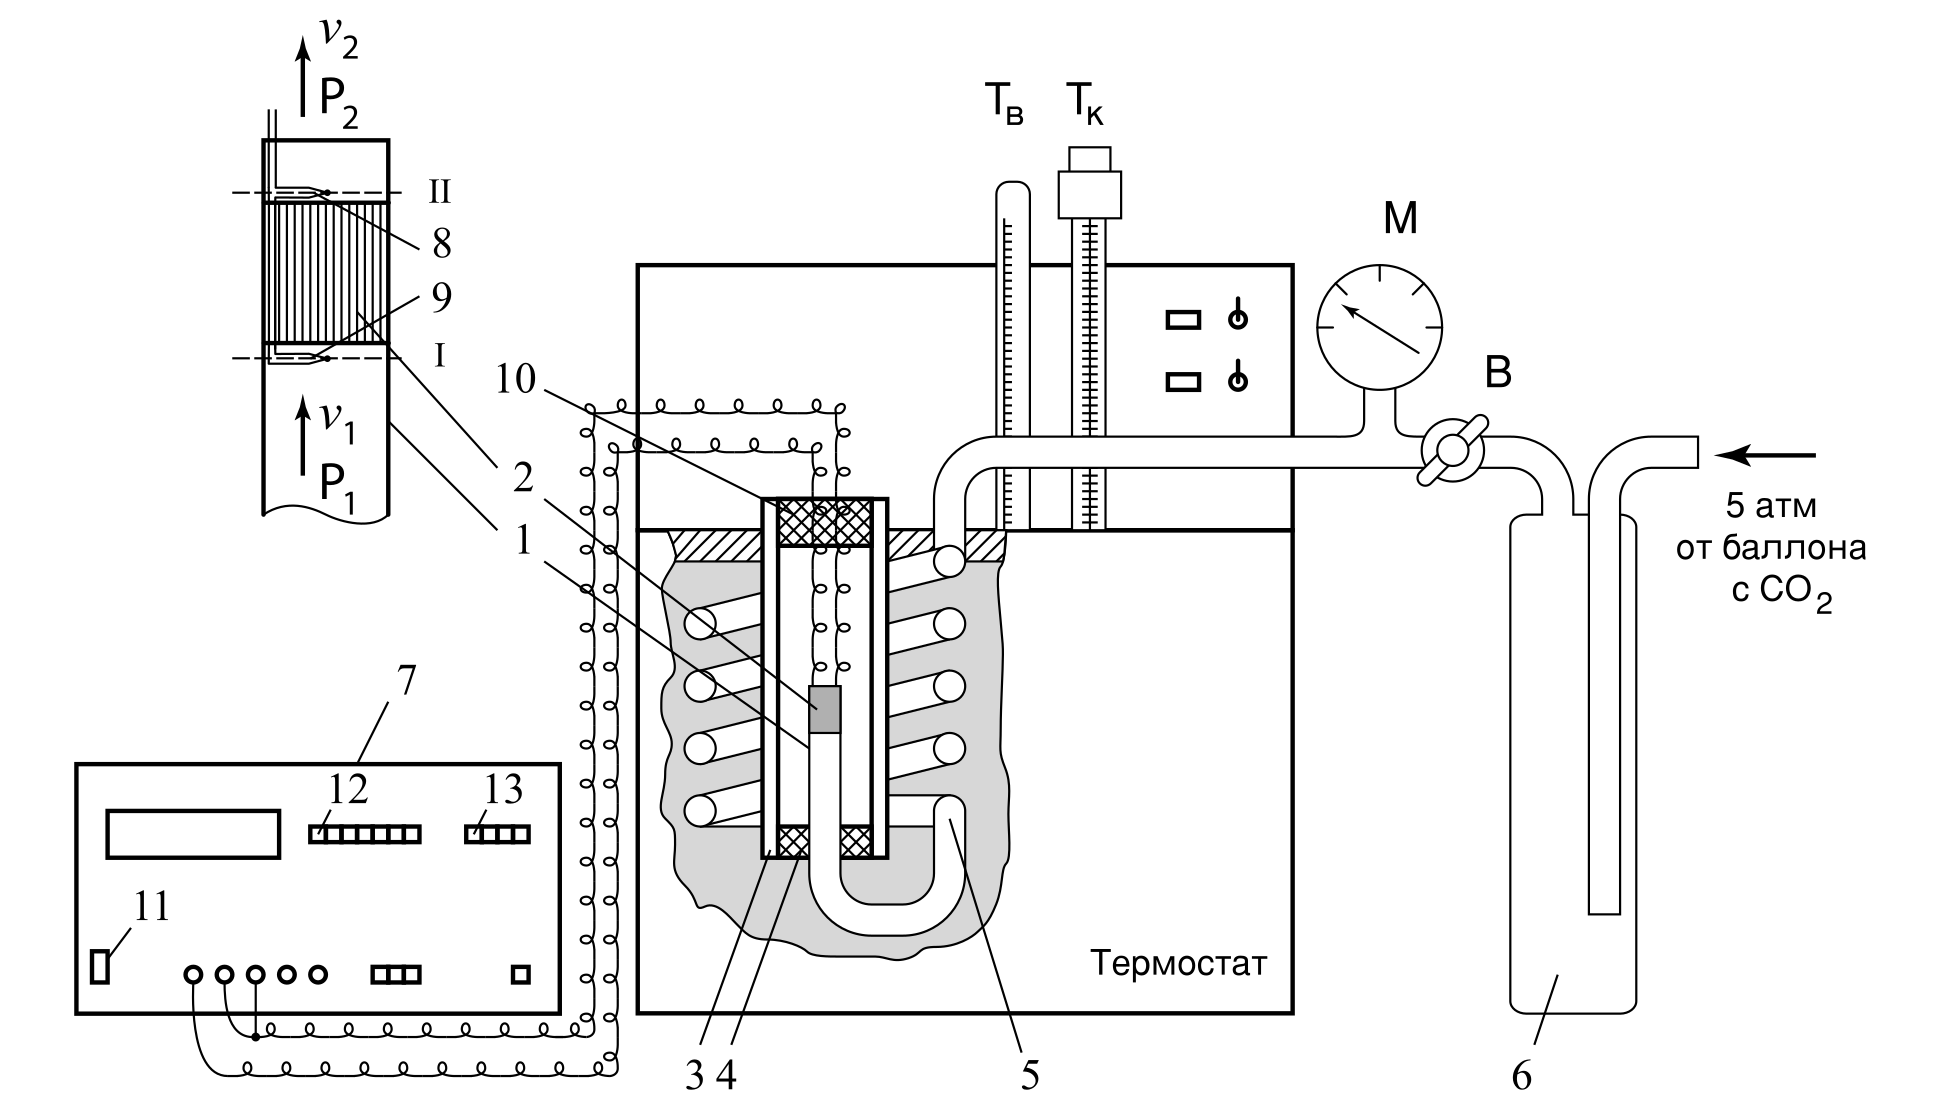
\includegraphics[scale=0.2]{PIC_1}
		\\\textbf{Рис. 1:} Схема установки
	\end{center}
		
	В работе исследуется изменение температуры углекислого газа	при медленном его течении по трубке с пористой перегородкой (Рис. 1). Трубка 1 хорошо теплоизолирована. Газ из области повышенного давления $P_1$ проходит через множество узких и длинных каналов пористой перегородки 2 в область с атмосферным давлением $P_2$. Перепад давления $\Delta P = P_2 - P_1$ из-за большого сопротивления каналов может быть заметным даже при малой скорости течения газа в трубке. Величина эффекта Джоуля–Томсона определяется по
	разности температуры газа до и после перегородки.	
		
	\textbf{В работе используются:}
	
	трубка с пористой перегородкой, труба Дьюара, термостат, термометры, дифференциальная термопара, микровольтметр, балластный баллон, манометр.
	
	\section{Теоретические сведения}
	Рассмотрим стационарный поток газа между произвольными сечениями $I$ и $II$ трубки (до перегородки и после нее). Пусть, для определенности, через трубку прошел 1 моль углекислого газа; $\mu$ -- его
	молярная масса. Молярные объемы газа, его давления и отнесенные	к молю внутренние энергии газа в сечениях $I$ и $II$ обозначим соответственно $V_1$, $P_1$ , $U_1$ и $V_2$, $P_2$, $U_2$. Для того чтобы ввести в трубку объем $V_1$, над газом нужно совершить работу $A_1 = P_1 V_1$. Проходя через сечение $II$, газ сам совершает работу $A_2 = P_2 V_2$. Так как через боковые стенки не происходит ни обмена теплом, ни передачи механической энергии, то:
	
	\newpage 
	
	%Страница 3
	
	\begin{flushleft}
		\footnotesize{Эффект Джоуля-Томсона} \hspace{\fill} \footnotesize{3}
		\\[-0.3cm]\noindent\rule{\textwidth}{0.3pt}
	\end{flushleft}
	
	\begin{equation}
		A_1 - A_2 = \left(U_2 + \sfrac{\mu\upsilon_2^2}{2}\right) - \left(U_1 + \sfrac{\mu \upsilon_1^2}{2}\right)
	\end{equation}
	
	В уравнении (1) учтено изменение как внутренней (первые члены в	скобках), так и кинетической (вторые члены в скобках) энергии газа. Подставляя в (1) написанные выражения для $A_1$ и $A_2$ и перегруппировывая члены, найдем
	
	\begin{equation}
		H_1 - H_2 = (U_1 + P_1V_1) - (U_2 + P_2V_2) = \sfrac{1}{2}\mu(\upsilon_1^2 - \upsilon_2^2)
	\end{equation}
	
	Сделаем несколько замечаний. Прежде всего отметим, что в процессе Джоуля–Томсона газ испытывает в пористой перегородке существенное трение, приводящее к ее нагреву. Потери энергии на нагрев	трубки в начале процесса могут быть очень существенными и сильно	искажают ход явления. После того как температура трубки установится и газ станет уносить с собой все выделенное им в пробке тепло, формула (1) становится точной, если, конечно, теплоизоляция трубки достаточно хороша и не происходит утечек тепла наружу через ее стенки.
	
	Второе замечание связано с правой частью (2). Процесс Джоуля–Томсона в чистом виде осуществляется лишь в том случае, если правой частью можно пренебречь, т. е. если макроскопическая скорость газа с обеих сторон трубки достаточно мала. У нас сейчас	нет критерия, который позволил бы установить, когда это можно сделать. Поэтому мы отложим на некоторое время обсуждение вопроса	о правой части (2), а пока будем считать, что энтальпия газа не меняется.
	
	\begin{equation}
		\mu_{\text{д-т}} = \sfrac{\Delta T}{\Delta P} \approx \sfrac{2a/RT - b}{C_p}
	\end{equation}

	Из формулы (3) видно, что эффект Джоуля–Томсона для не очень плотного газа зависит от соотношения величин $a$ и $b$, которые оказывают противоположное влияние на знак эффекта. Если силы взаимодействия между молекулами велики, так что превалирует «поправка на давление», то основную роль играет член, содержащий $a$, и
	
	$$\sfrac{\Delta T}{\Delta P} > 0$$
	
	т. е. газ при расширении охлаждается ($\Delta T < 0$, так как всегда $\Delta P < 0$). В обратном случае (малые $a$)
	
	$$\sfrac{\Delta T}{\Delta P} < 0$$

	т. е. газ нагревается ($\Delta T > 0$, так как по-прежнему $\Delta P < 0$).	Этот результат нетрудно понять из энергетических соображений. Как мы уже знаем, у идеального газа эффект Джоуля–Томсона отсутствует. Идеальный газ отличается от реального тем, что в нем можно	пренебречь потенциальной энергией взаимодействия молекул. Наличие этой энергии приводит к охлаждению или нагреванию реальных газов при расширении. При больших $a$ велика энергия притяжения	молекул. Это означает, что потенциальная энергия молекул при их сближении уменьшается, а при удалении — при расширении газа — возрастает. Возрастание потенциальной энергии молекул происходит за счет их кинетической энергии — температура газа при расширении	падает. Аналогичные рассуждения позволяют понять, почему расширяющийся газ нагревается при больших значениях $b$.
	
	\newpage 
	
	%Страница 4
	
	\begin{flushleft}
		\footnotesize{Эффект Джоуля-Томсона} \hspace{\fill} \footnotesize{4}
		\\[-0.3cm]\noindent\rule{\textwidth}{0.3pt}
	\end{flushleft}
	
	При температуре $T_{\mathrm{inv}}$ эффект Джоуля–Томсона меняет знак: ниже температуры инверсии эффект положителен ($\mu_{\text{д-т}} > 0$, газ охлаждается), выше $T_{\mathrm{inv}}$ эффект отрицателен ($\mu_{\text{д-т}} < 0$, газ нагревается).

	\section{Проведение эксперимента}
	\paragraph{Измерение коэффициента Джоуля-Томсона} \hfill
	
	Представим в табличном виде зависимость $\Delta T (\Delta P)$, сразу пересчитав через таблицу чувствительности термопары $\Delta U$ в $\Delta T$.

	\begin{center}
		\begin{tabular}{|c|c|c|c|c|c|c|}
			\hline
			\multicolumn{7}{|c|}{$T$ = 291 К}
			\\\hline
			$\Delta P$, атм & $3.00 \pm 0.05$ & $2.60 \pm 0.05$ & $2.20 \pm 0.05$ & $1.80 \pm 0.05$ & $1.40 \pm 0.05$ & $1.00 \pm 0.05$
			\\\hline
			$U - U_0$, мкВ & $138 \pm 2$ & $120 \pm 2$ & $102 \pm 2$ & $85 \pm 2$ & $68 \pm 2$ & $55 \pm 2$
			\\\hline
			$\Delta T$, К & $3.47 \pm 0.05$ & $3.02 \pm 0.05$ & $2.56 \pm 0.05$ & $2.14 \pm 0.05$ & $1.71 \pm 0.05$ & $1.38 \pm 0.05$
			\\\hline
			\multicolumn{7}{|c|}{$T$ = 308 К}
			\\\hline
			$\Delta P$, атм & $3.00 \pm 0.05$ & $2.60 \pm 0.05$ & $2.20 \pm 0.05$ & $1.80 \pm 0.05$ & $1.40 \pm 0.05$ & $1.00 \pm 0.05$
			\\\hline
			$U - U_0$, мкВ & $115 \pm 2$ & $98 \pm 2$ & $82 \pm 2$ & $66 \pm 2$ & $51 \pm 2$ & $40 \pm 2$
			\\\hline
			$\Delta T$, К & $2.76 \pm 0.05$ & $2.36 \pm 0.05$ & $1.97 \pm 0.05$ & $1.59 \pm 0.05$ & $1.23 \pm 0.05$ & $0.96 \pm 0.05$
			\\\hline
			\multicolumn{7}{|c|}{$T$ = 333 К}
			\\\hline
			$\Delta P$, атм & $3.00 \pm 0.05$ & $2.60 \pm 0.05$ & $2.20 \pm 0.05$ & $1.80 \pm 0.05$ & $1.40 \pm 0.05$ & $1.00 \pm 0.05$
			\\\hline
			$U - U_0$, мкВ & $91 \pm 2$ & $80 \pm 2$ & $68 \pm 2$ & $55 \pm 2$ & $41 \pm 2$ & $28 \pm 2$
			\\\hline
			$\Delta T$, К & $2.10 \pm 0.05$ & $1.85 \pm 0.05$ & $1.57 \pm 0.05$ & $1.27 \pm 0.05$ & $0.95 \pm 0.05$ & $0.65 \pm 0.05$
			\\\hline
		\end{tabular}
		\\\textbf{Табл. 1:} Измерение коэффициента Джоуля-Томсона
	\end{center}

	Построим графики зависимостей для данных температур.
	
	\begin{center}
		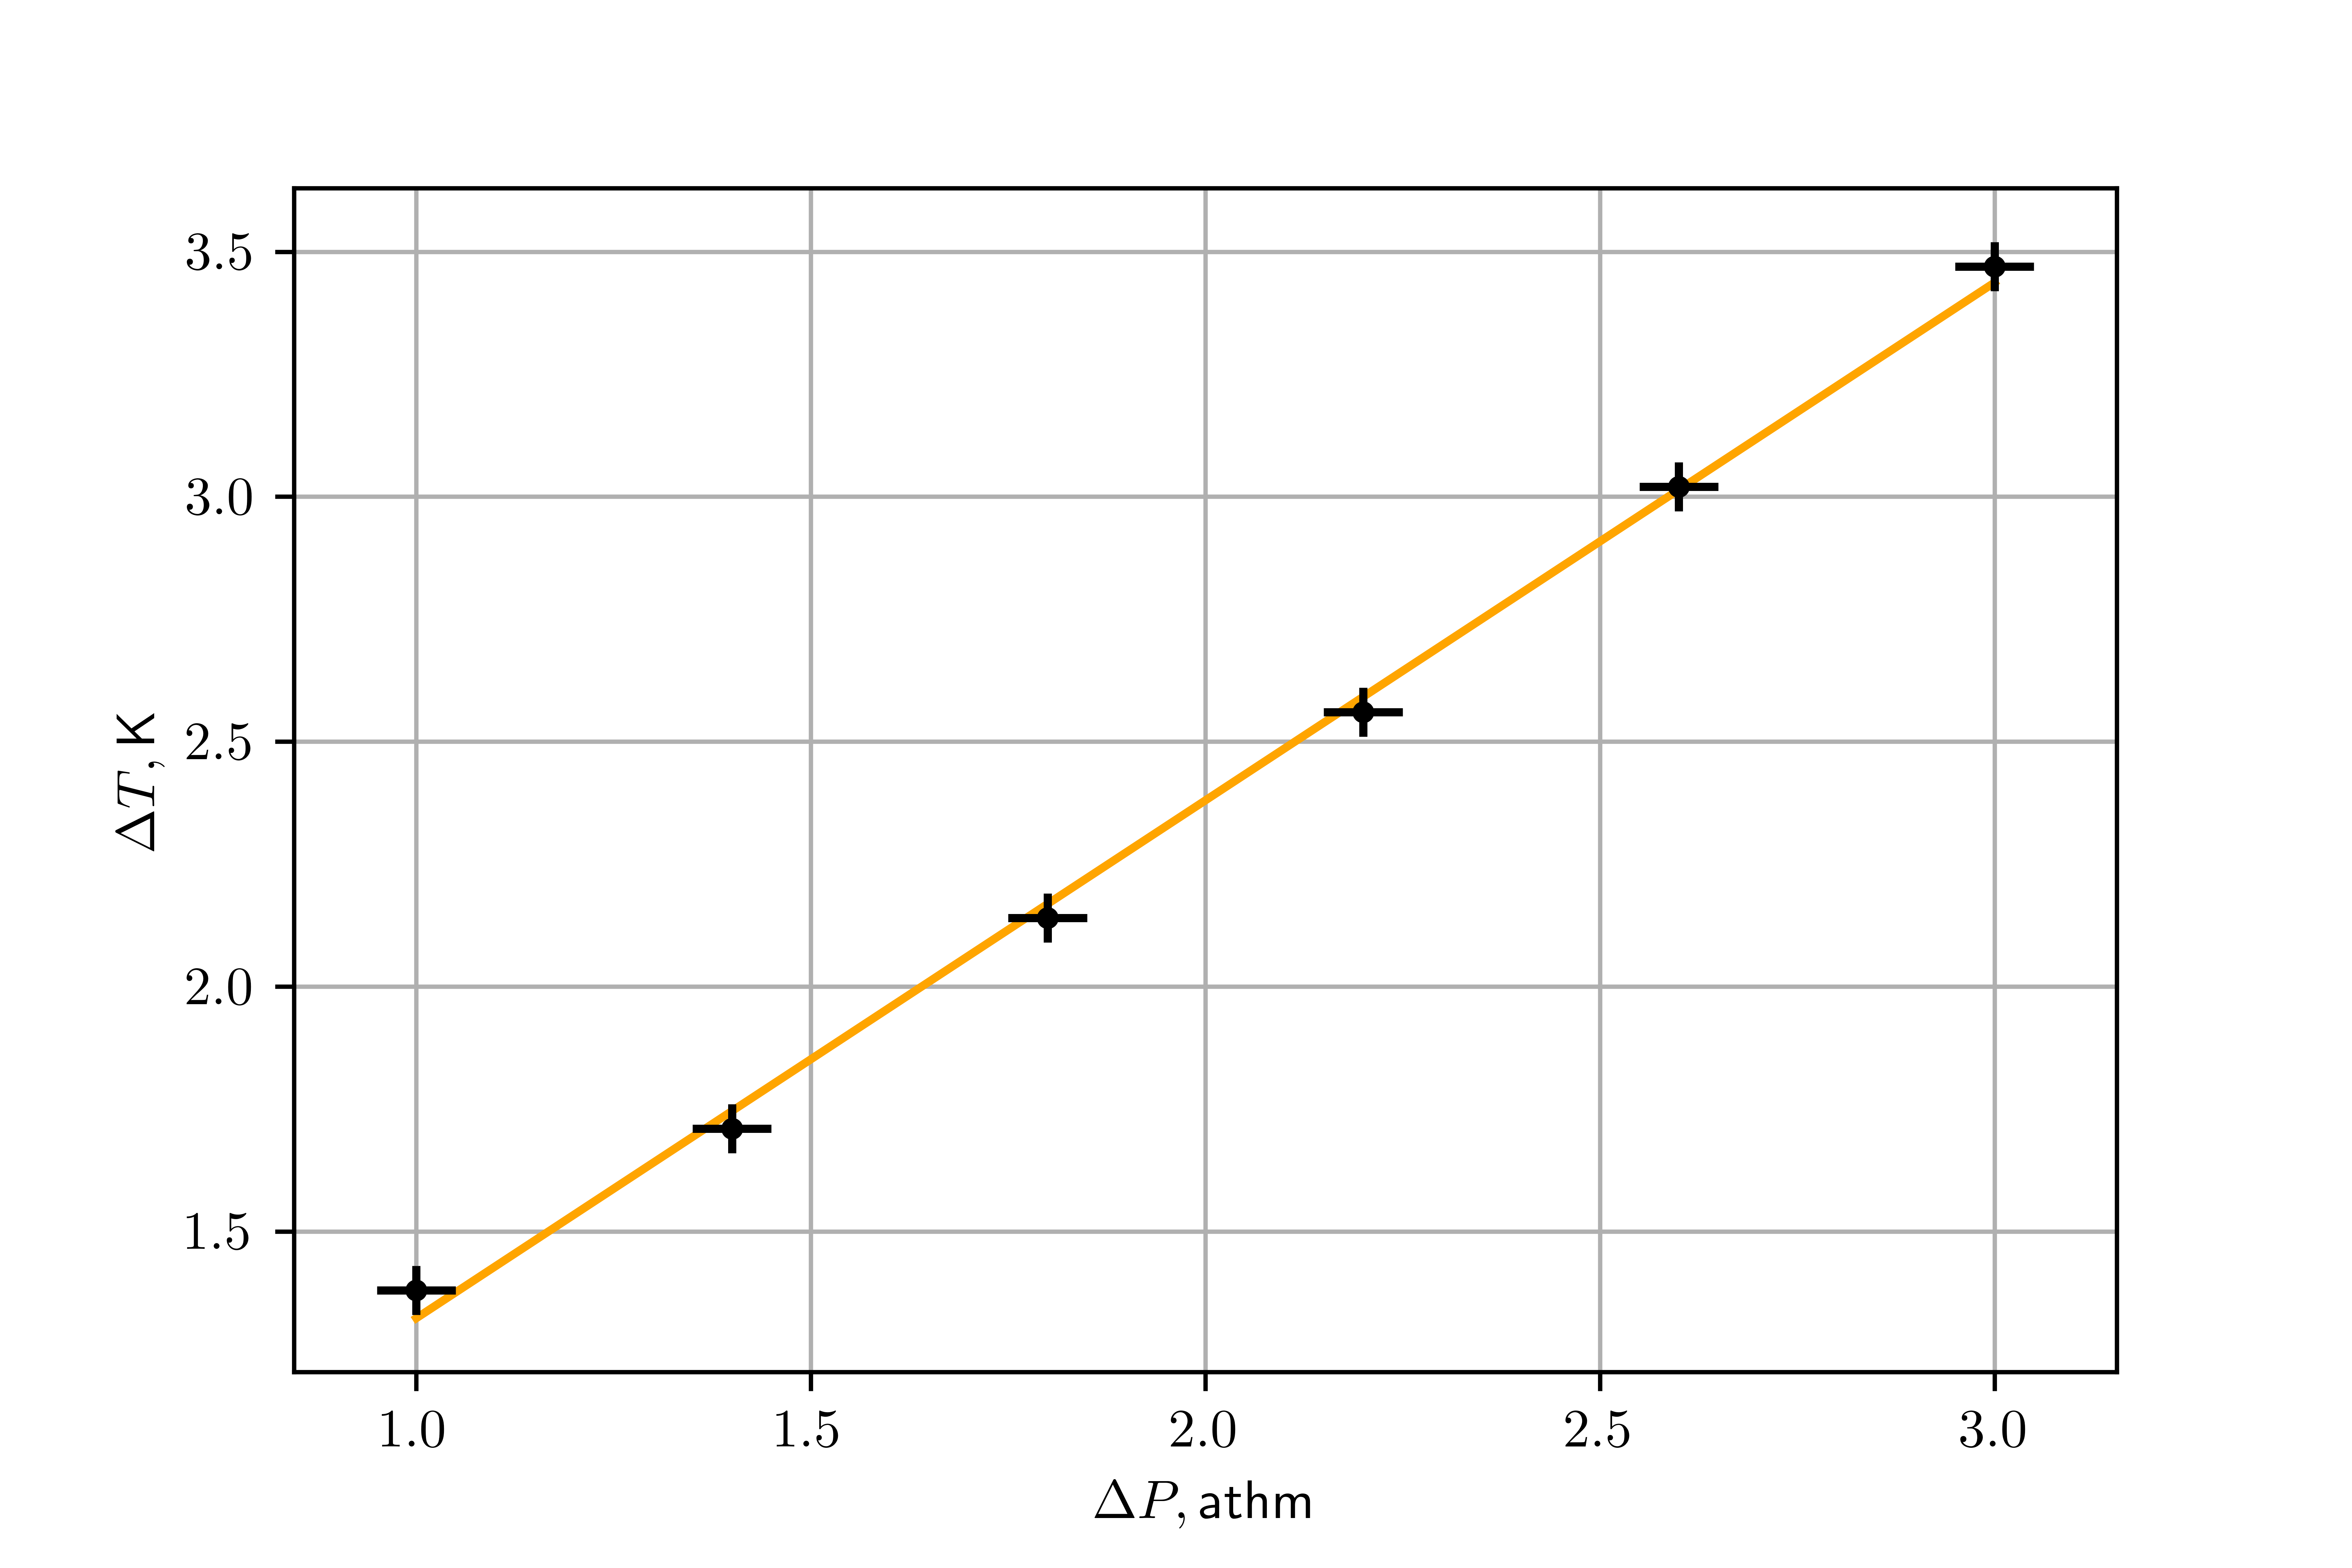
\includegraphics[scale=0.8]{PIC_2.png}
		\\\textbf{Рис. 2:} График зависимости $\Delta T (\Delta P)$ при $T = 291$ К
	\end{center}

	\newpage 
	
	%Страница 5
	
	\begin{flushleft}
		\footnotesize{Эффект Джоуля-Томсона} \hspace{\fill} \footnotesize{5}
		\\[-0.3cm]\noindent\rule{\textwidth}{0.3pt}
	\end{flushleft}

	\begin{center}
		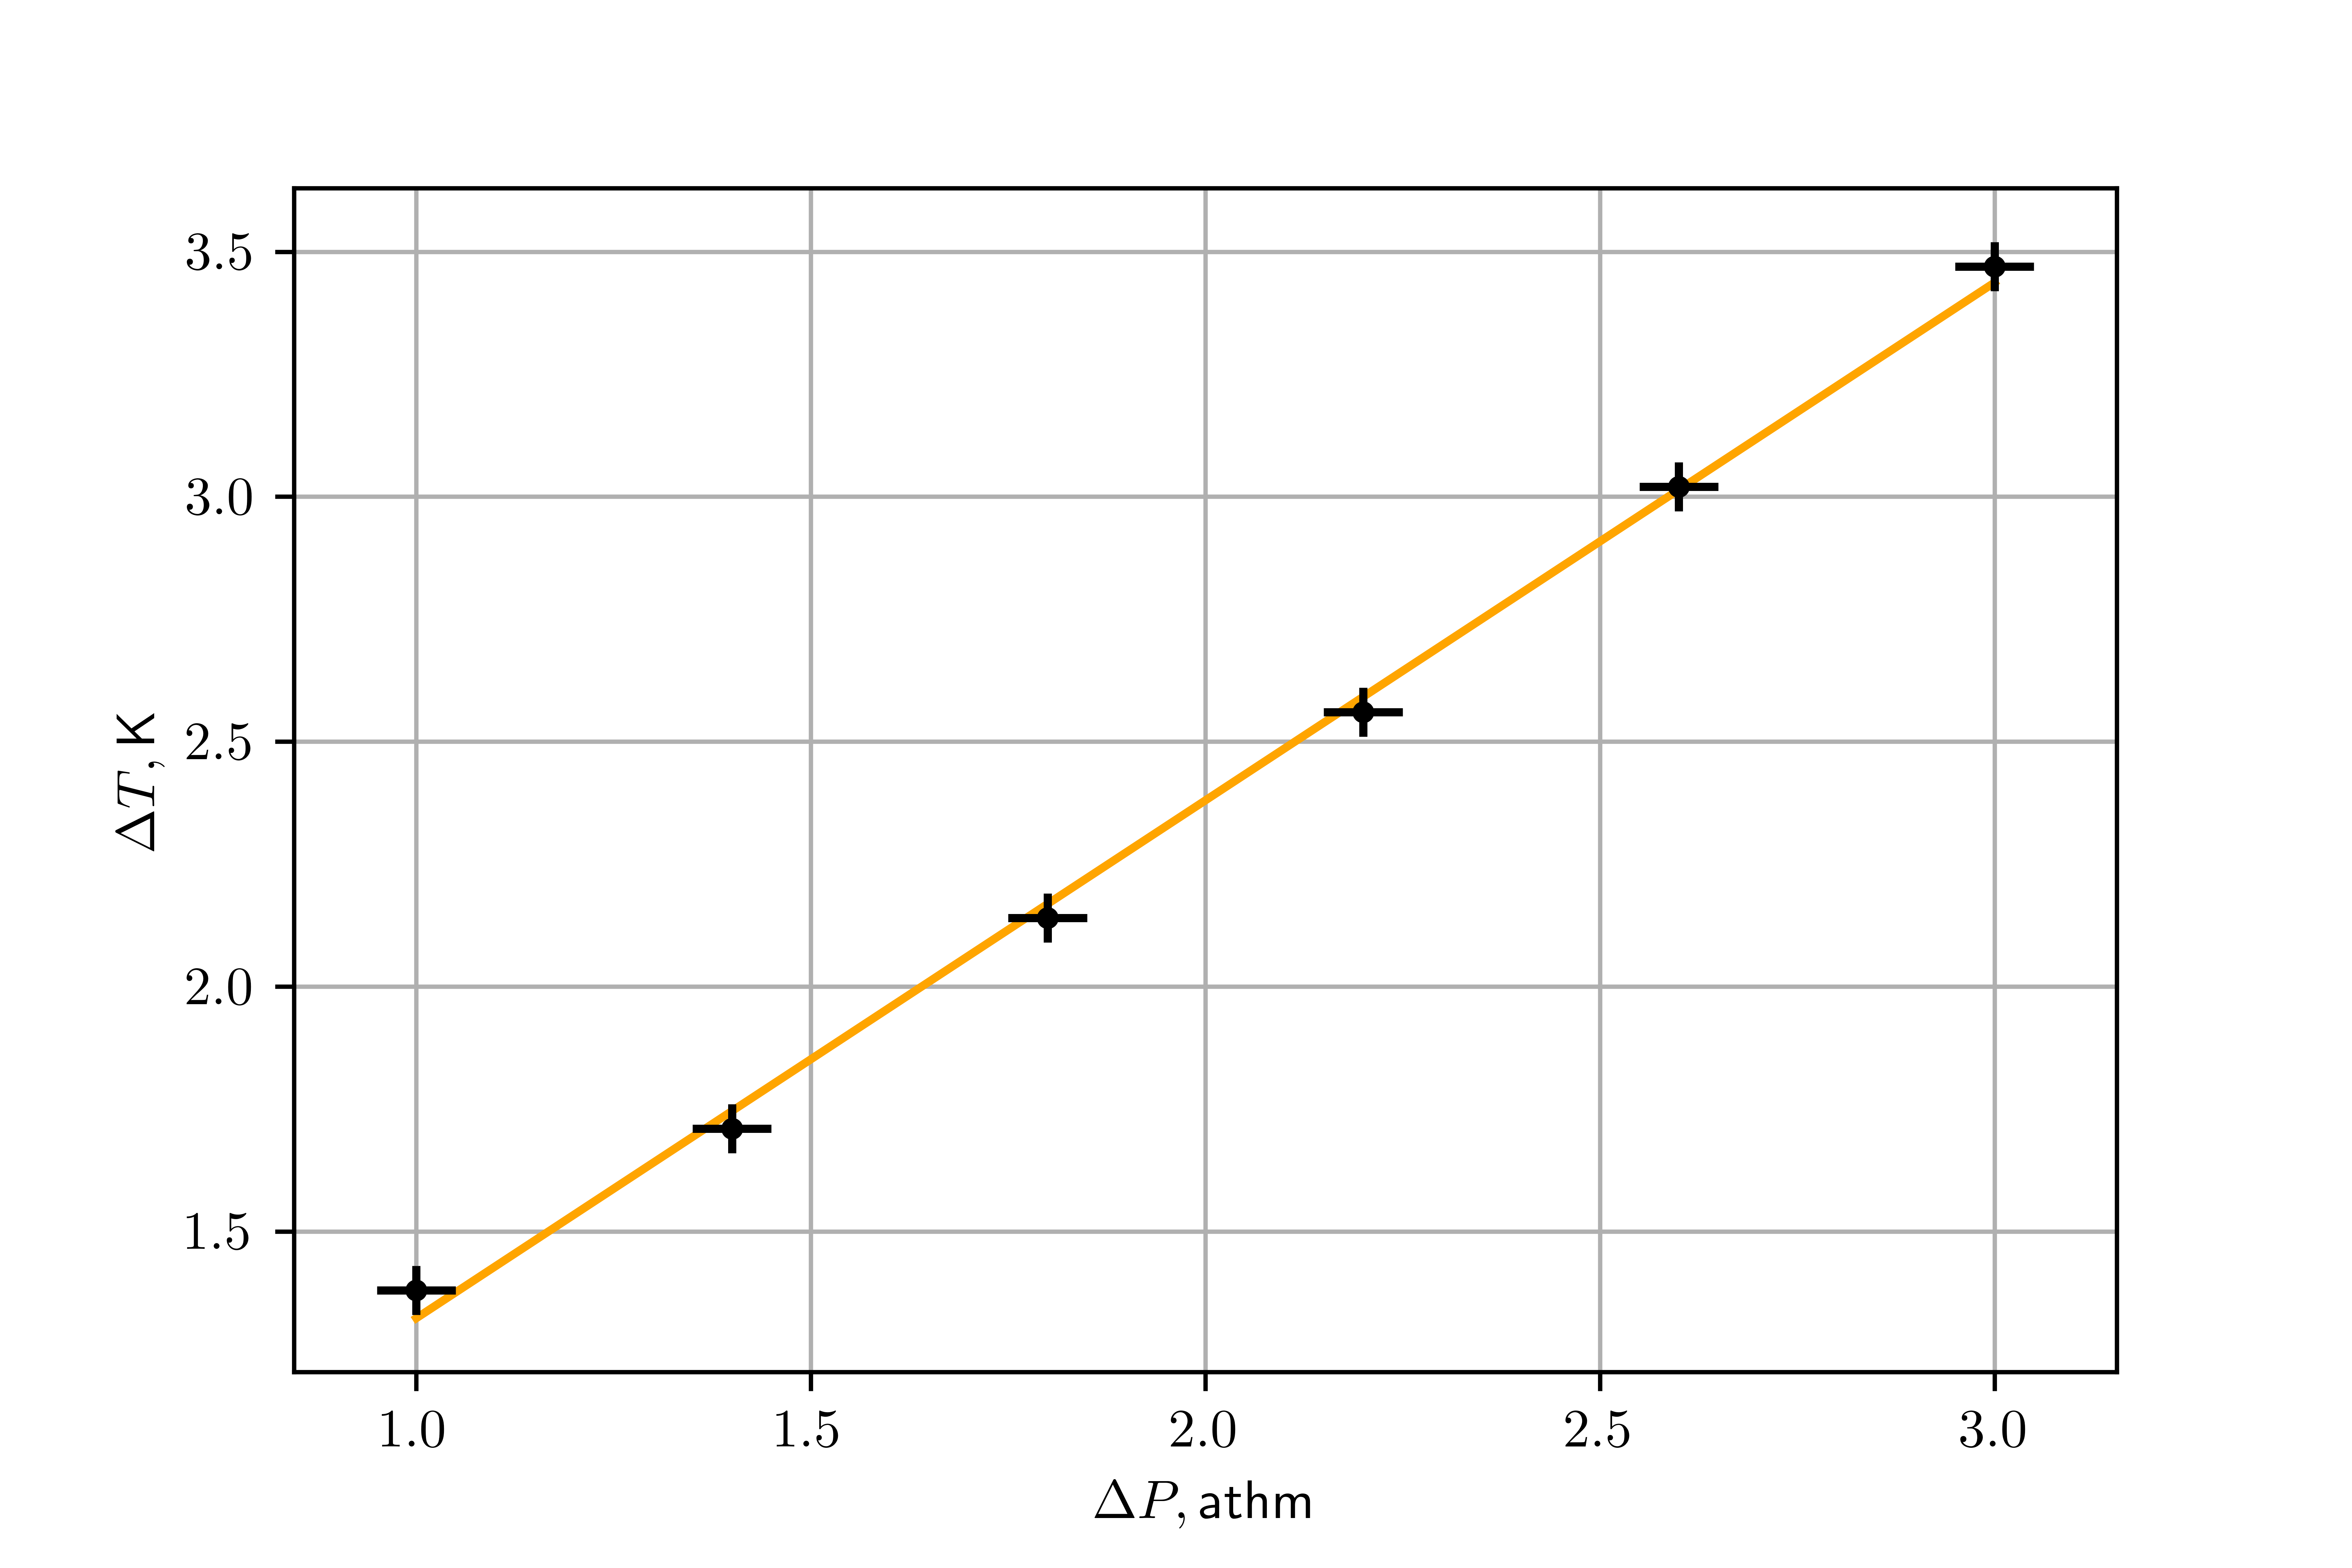
\includegraphics[scale=0.8]{PIC_2.png}
		\\\textbf{Рис. 3:} График зависимости $\Delta T (\Delta P)$ при $T = 308$ К
	\end{center}

	\begin{center}
		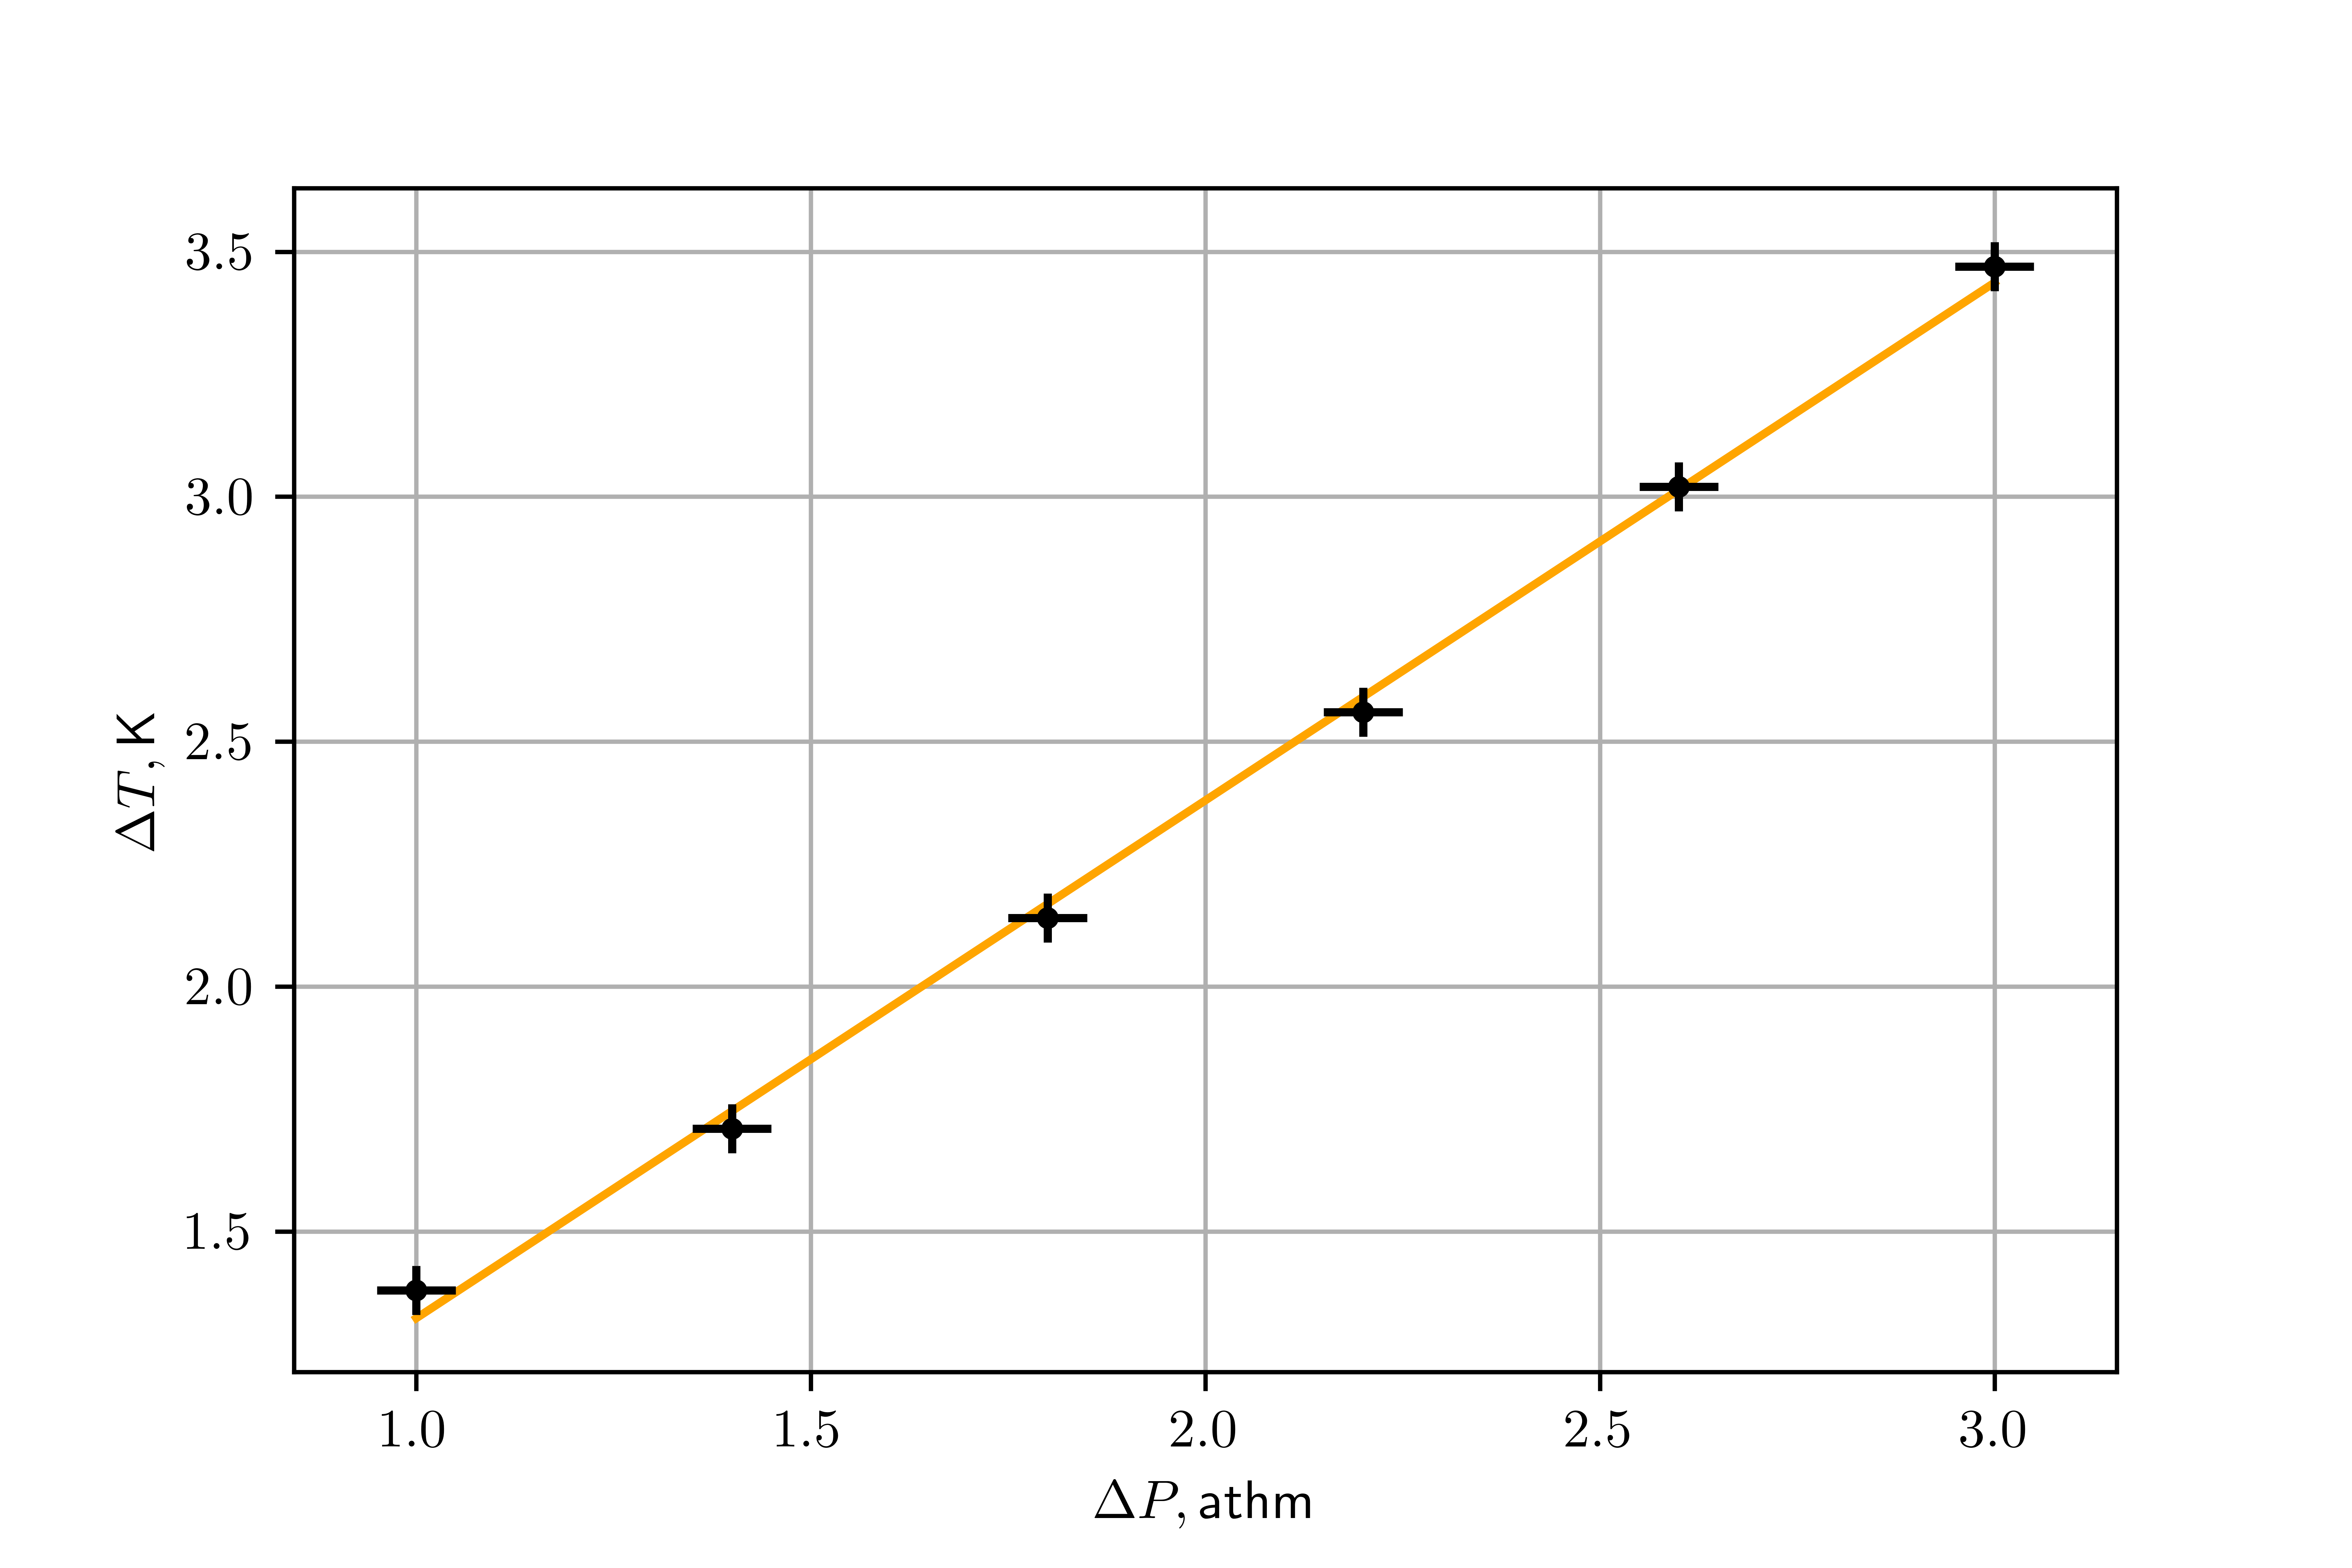
\includegraphics[scale=0.8]{PIC_2.png}
		\\\textbf{Рис. 4:} График зависимости $\Delta T (\Delta P)$ при $T = 333$ К
	\end{center}

	Теперь рассчитаем соответствующие коэффициенты Джоуля-Томсона и занесем их в таблицу:
	
	\begin{center}
		\begin{tabular}{|c|c|c|c|}
			\hline
			$T$, К & 291 & 308 & 333
			\\\hline
			$\mu_{\text{д-т}}$, К/атм & $1.06 \pm 0.03$ & $0.91 \pm 0.02$ & $.73 \pm 0.01$
			\\\hline
		\end{tabular}
	\end{center}

	\paragraph{Рассчет коэффициентов Ван-дер-Ваальса} \hfill

	По данным таблицы 2 построим график зависимости $\mu_{\text{д-т}}(1/T)$ и рассчитаем необходимые значения.
	
	\newpage 
	
	%Страница 6
	
	\begin{flushleft}
		\footnotesize{Эффект Джоуля-Томсона} \hspace{\fill} \footnotesize{6}
		\\[-0.3cm]\noindent\rule{\textwidth}{0.3pt}
	\end{flushleft}
	
	\begin{center}
		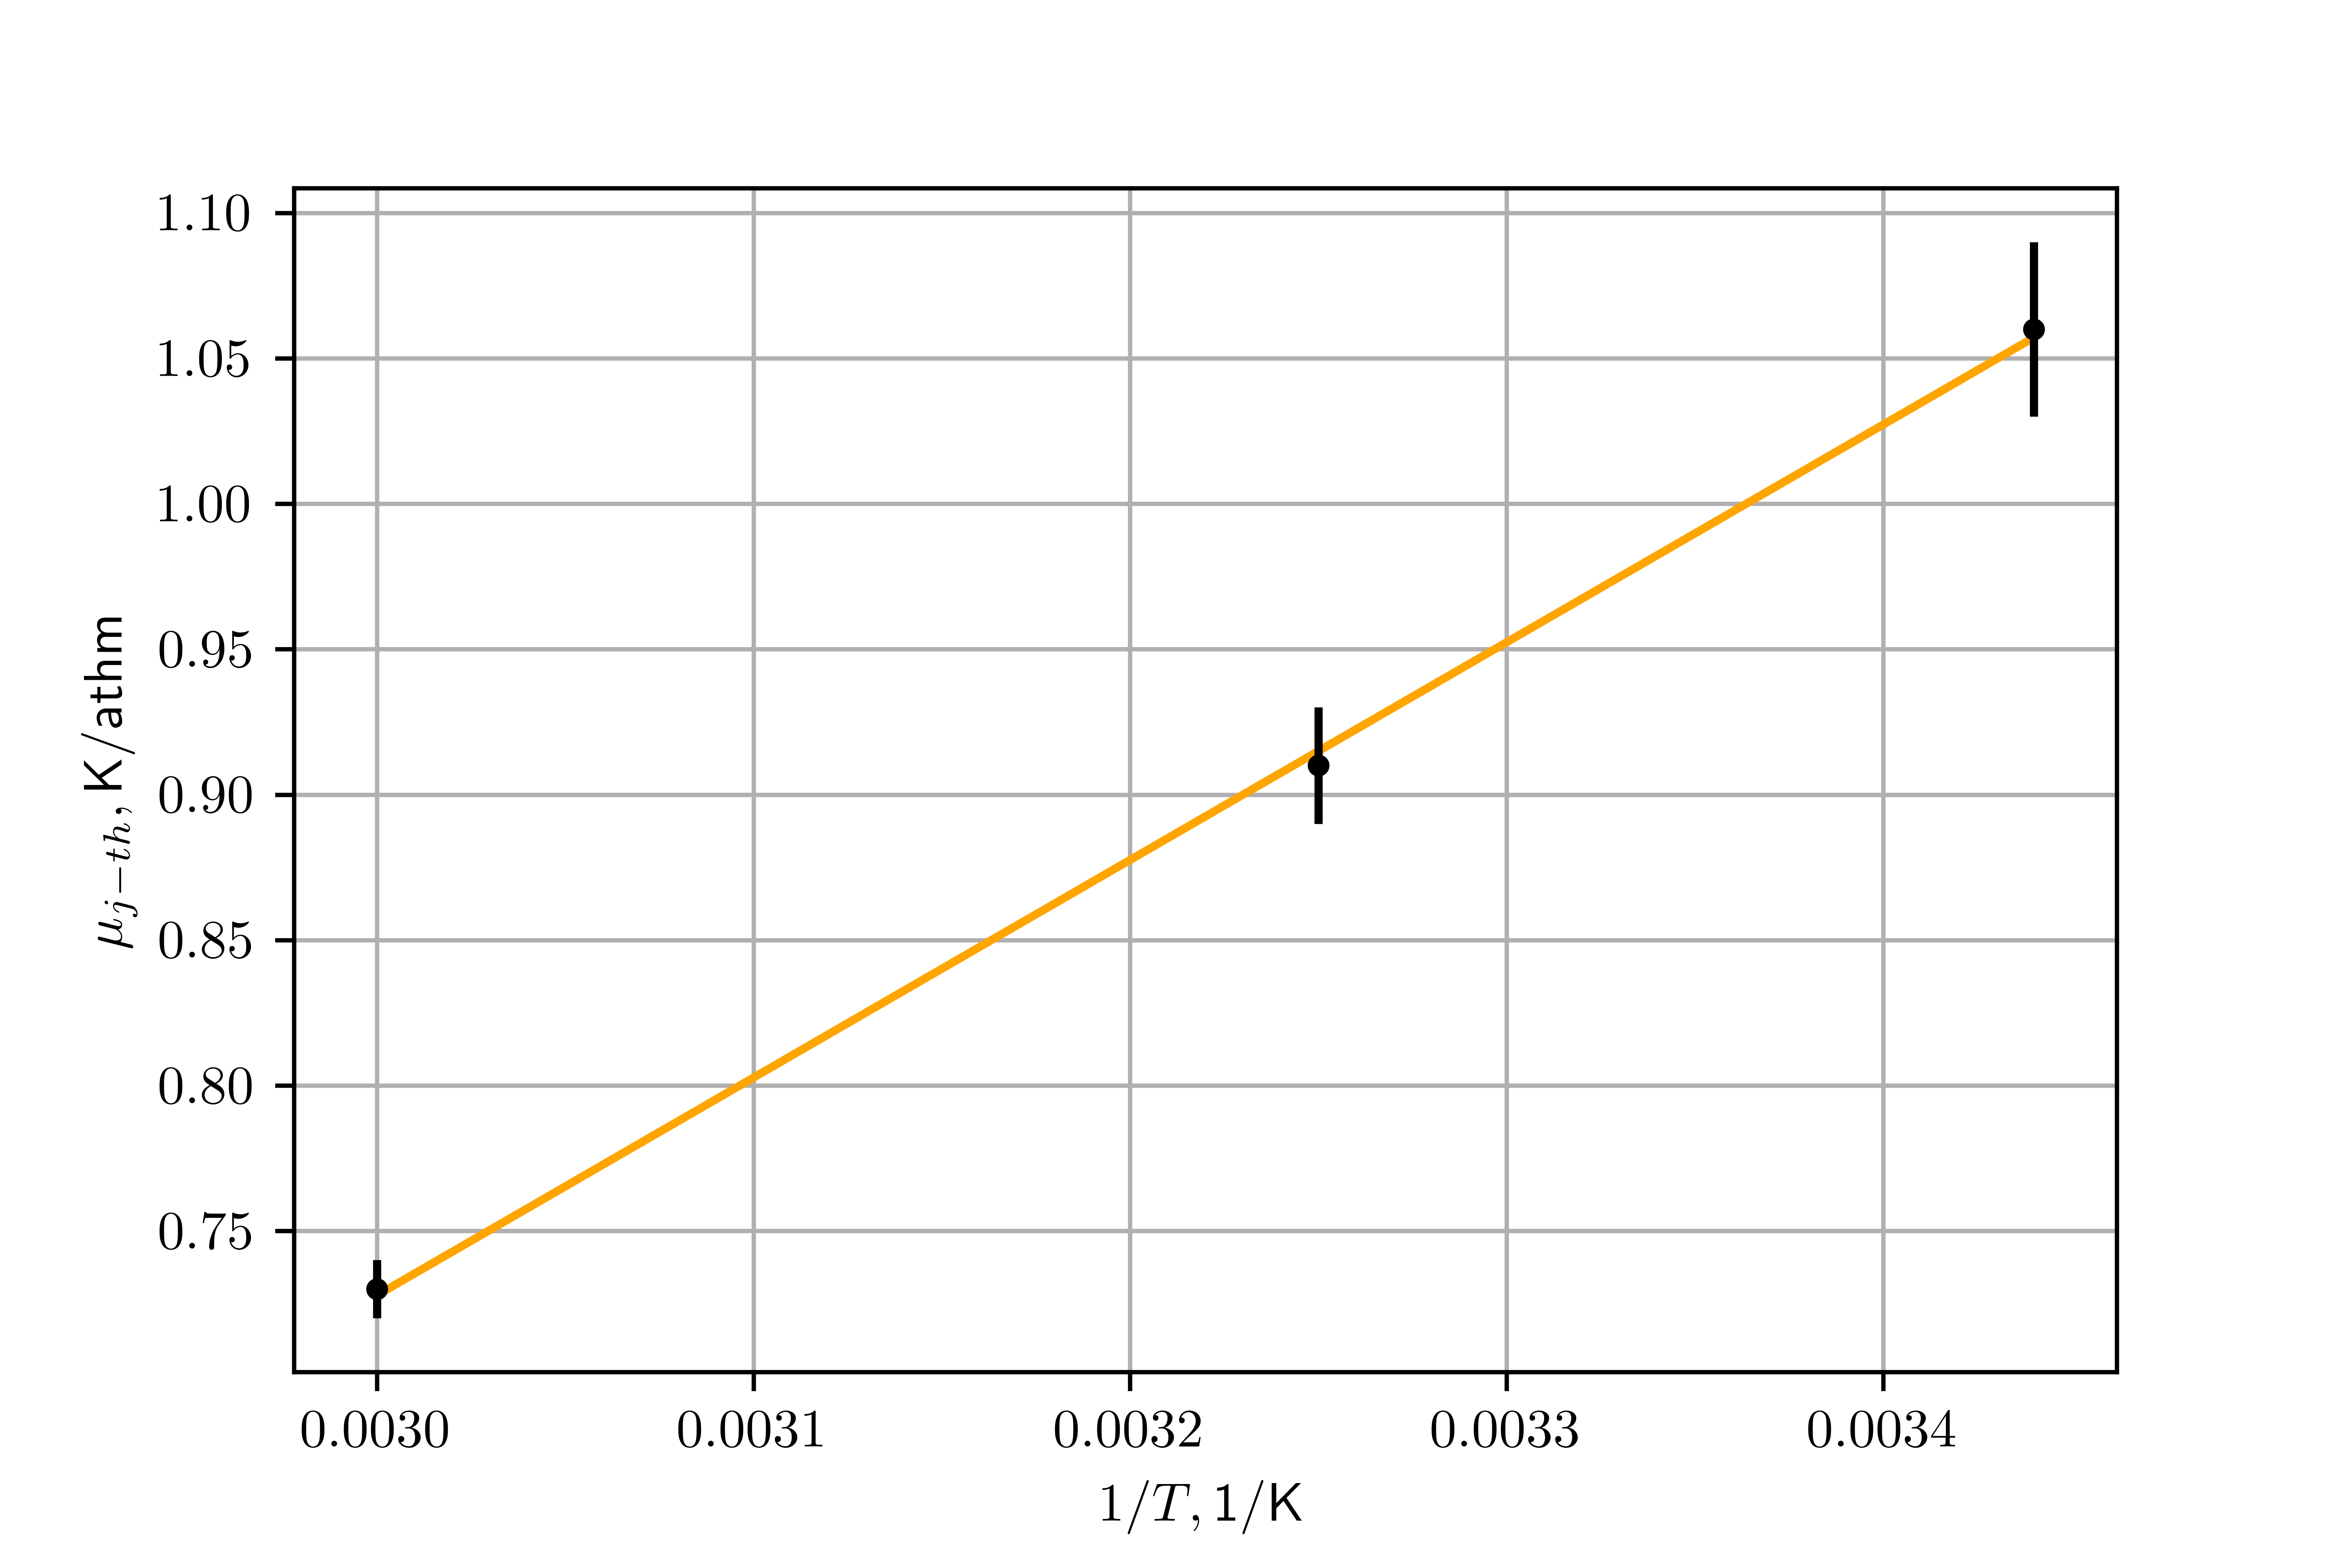
\includegraphics[scale=0.8]{PIC_5}
		\\\textbf{Рис. 5}: График зависимости $\mu_{\text{д-т}}(1/T)$
	\end{center}
	
	Отсюда получаем параметры нашего графика $\mathrm{slope} = (75 \pm 2) \cdot 10^{-4}$ К$^2$/Па, $\mathrm{intercept} = (-1.52 \pm 0.06) \cdot 10^{-5}$ 1/К.
	
	$$a = \sfrac{\mathrm{slope} \cdot RC_p}{2} = 1.28 \pm 0.03\ \sfrac{\text{Н} \cdot \text{м}^4}{\text{моль}^2}$$
	
	$$b = -\mathrm{intercept} \cdot C_p = (6.2 \pm 0.2) \cdot 10^{-4}\ \sfrac{\text{м}^3}{\text{моль}}$$
	
	$$T_{\mathrm{inv}} = \sfrac{2a}{Rb} = 497 \pm 19\ \text{К}$$
	
	\section{Выводы}
	\begin{enumerate}
		\item В результате работы определены коэффициенты Ван-дер-Ваальса для углекислого газа:
		
		$$a = \sfrac{\mathrm{slope} \cdot RC_p}{2} = 1.28 \pm 0.03\ \sfrac{\text{Н} \cdot \text{м}^4}{\text{моль}^2}$$
		
		$$b = -\mathrm{intercept} \cdot C_p = (6.2 \pm 0.2) \cdot 10^{-4}\ \sfrac{\text{м}^3}{\text{моль}}$$
		
		\item Получено значение инверсной температуры Джоуля-Томсона для углекислого газа:
		
		$$T_{\mathrm{inv}} = \sfrac{2a}{Rb} = 497 \pm 19\ \text{К}$$
			
		При этом табличное значение $T_{\mathrm{inv}\ 0} = 2027 \text{К}$.
	\end{enumerate}
	
	
	Таким образом, можно сделать вывод, что уравнение Ван-дер-Ваальса дает хорошую качественную модель реального газа, но конкретные численные значения коэффициентов верны лишь в узком диапазоне температур.
\end{document}